\begin{figure}
    \centering
    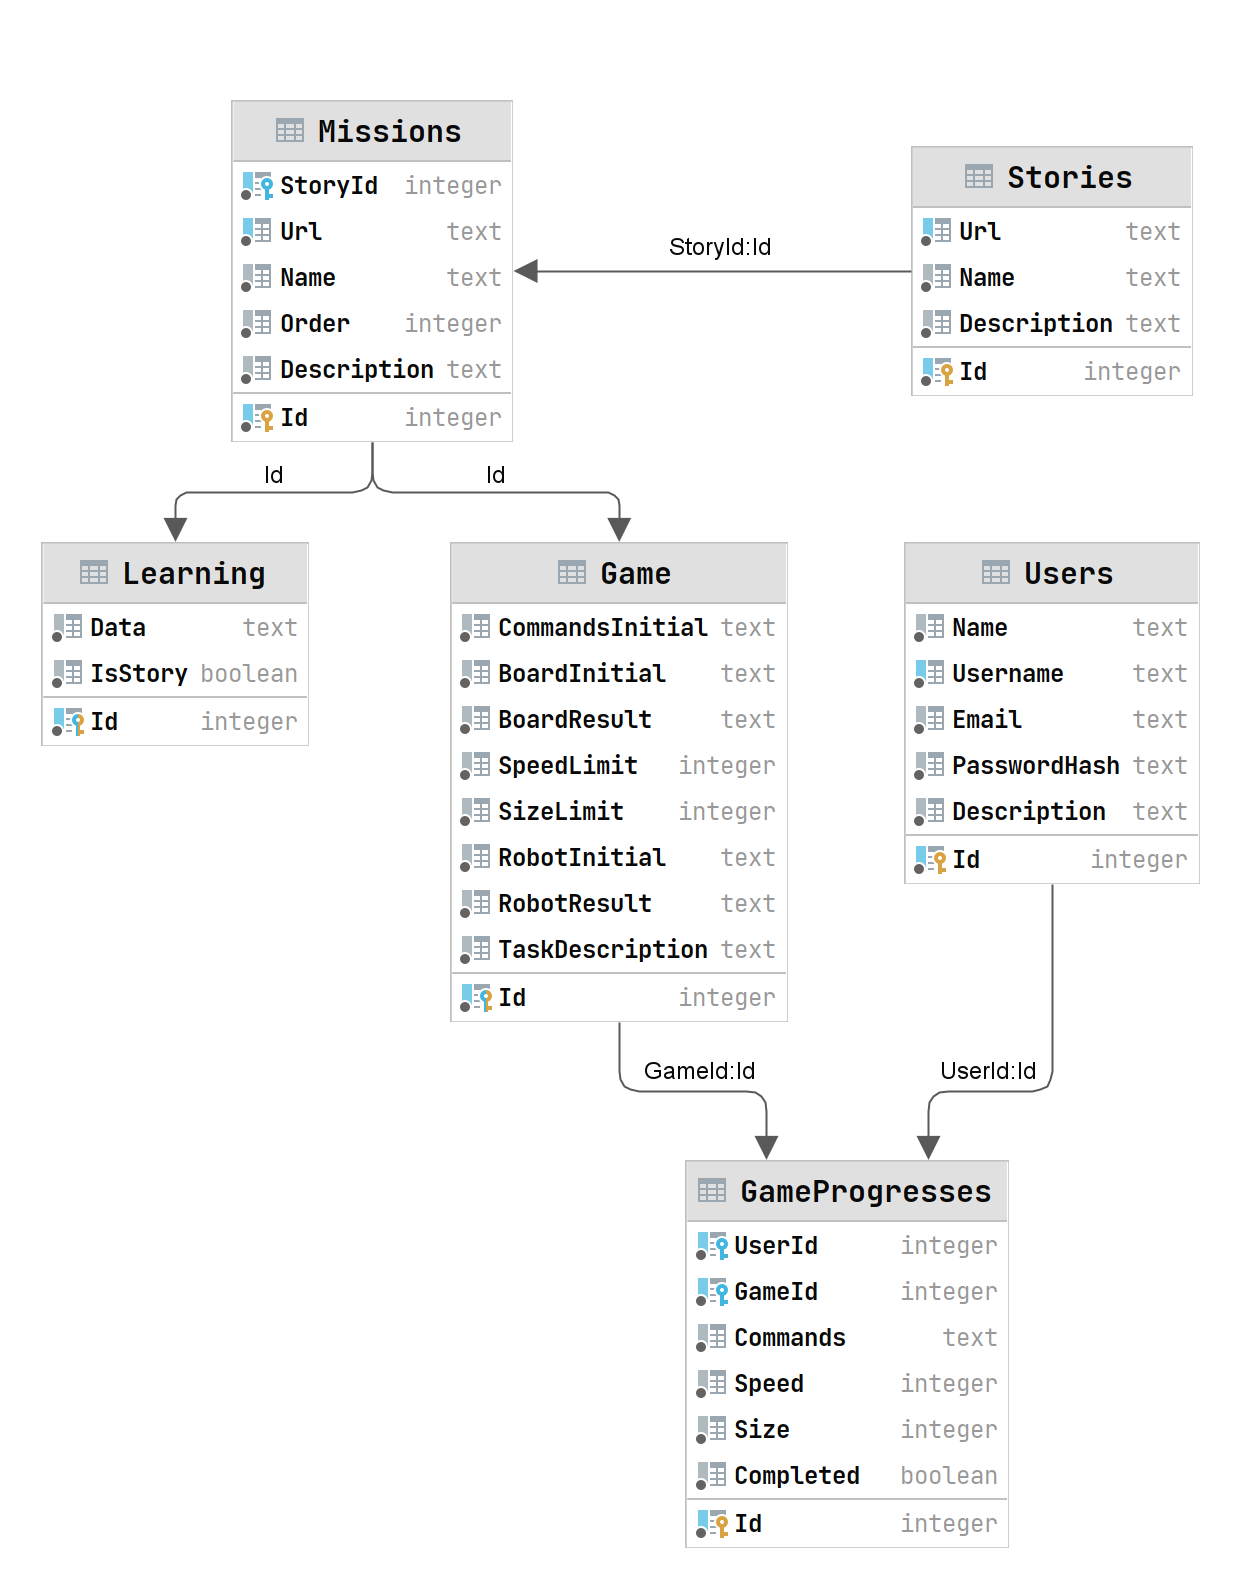
\includegraphics[width=1\linewidth]{assets/implementation/erdiagram.png}
    \caption{Relational Schema}
    \label{fig:impementation:relationalschema}
\end{figure}

\begin{listing}
    \caption{Entity Framework Migration Tools}
    \label{listing:migration}
    \begin{minted}{shell}
# installation
dotnet tool install --global dotnet-ef

# create a migration
cd KingKarel
dotnet ef migrations add "Name of migration"

# update the database
dotnet ef database update
    \end{minted}
\end{listing}

\section{Database}

According to the design chapter \ref{chapter:design}, the PostgreSQL was used as a database for the game.
For local development, a docker container with the database is set up.
The docker-compose file is located in the server application project.

In the chapter \ref{design:conceptual} a conceptual schema is described.
According to that schema, a relational schema was created.
The relational schema can be seen in the figure \ref{fig:impementation:relationalschema}.
The strucute of relational schema is similar to the structure of the conceptual schema.
For unique identifiers integer data types are used.
For other attributes an integer, a string, or a boolean data types are used.
Inside some of the string attributes an encoded JSONs are stored.

\subsection{Migrations}

Migrations manage the database from the server application.
Entity framework tools support the creation and updates of migrations.
That is useful, especially when the database schema is created using the ORM from the code.
Each migration create a file with the \mintinline{text}|Up()| and \mintinline{text}|Down()| methods.
These methods allow migration tools to apply and undo a migration.
Migration files are generated to \mintinline{text}|KingKarel/Migrations| directory.
Useful migration tool's commands can be seen in the code \ref{listing:migration}.
